\documentclass[twocolumn]{aastex631}
\newcommand{\vdag}{(v)^\dagger}
\newcommand\aastex{AAS\TeX}
\newcommand\latex{La\TeX}
\usepackage{lipsum}
\begin{document}

\title{Research Proposal}

\author{Swapnaneel Dey}
\affiliation{Astronomy Department, University of Arizona}


\section{Introduction}
Cold dark matter halo potential wells actively drive galaxy formation as they accrete and cool surrounding gas. This process allows us to predict a strong correlation between galactic properties, such as stellar mass and luminosity, with the halo mass \citep{Girelli+2020}. For example, the stellar-to-halo mass (SHMR) relation provides ample information on galaxy formation and evolution. Since Dark matter halos grow their mass by merging with other such halos, it raises the question of whether the dark matter halo of the merger remnant follows the same evolutionary path as a dark matter halo of an isolated galaxy.

It is widely accepted that a significant and ubiquitous process that fuels galaxy evolution is through galaxy mergers. Most massive galaxies are formed by smaller and also other massive galaxies falling into their gravitational potential wells. It is, therefore, imperative to study the evolution of the dark matter halos through the mergers. The results of the study can help constrain various physical processes involved in galaxy mergers, such as feedback mechanisms and how efficiently baryonic matter converts into stars and galaxy assembly. 

Though the Halo-Halo merger has been well constrained, the galaxy-galaxy mergers relative to halo-halo mergers remain largely unexplored \citep{Hopkins+2010}. Various cosmological hydrodynamical galaxy simulations show that most of the stellar material in massive galaxies is a product of major mergers (merging with a similar massive galaxy) and orbiting satellites \citep{RG+2016}. Although there have been various studies in understanding the merger histories \citep{Hao+2022, Ramos+2022}, not much has been done to study the stellar remanent of Milky Way (MW), M31 type galaxies. Figure \ref{fig:merger statistics} shows that about 30 percent of simulated MW/M31 type galaxies go through at least one major merger since z = 1 \citep{Ramos+2022}. This motivates us to understand the Galaxy-Halo connection of stellar remnants of major mergers.
\begin{figure}[h!]
    \centering
    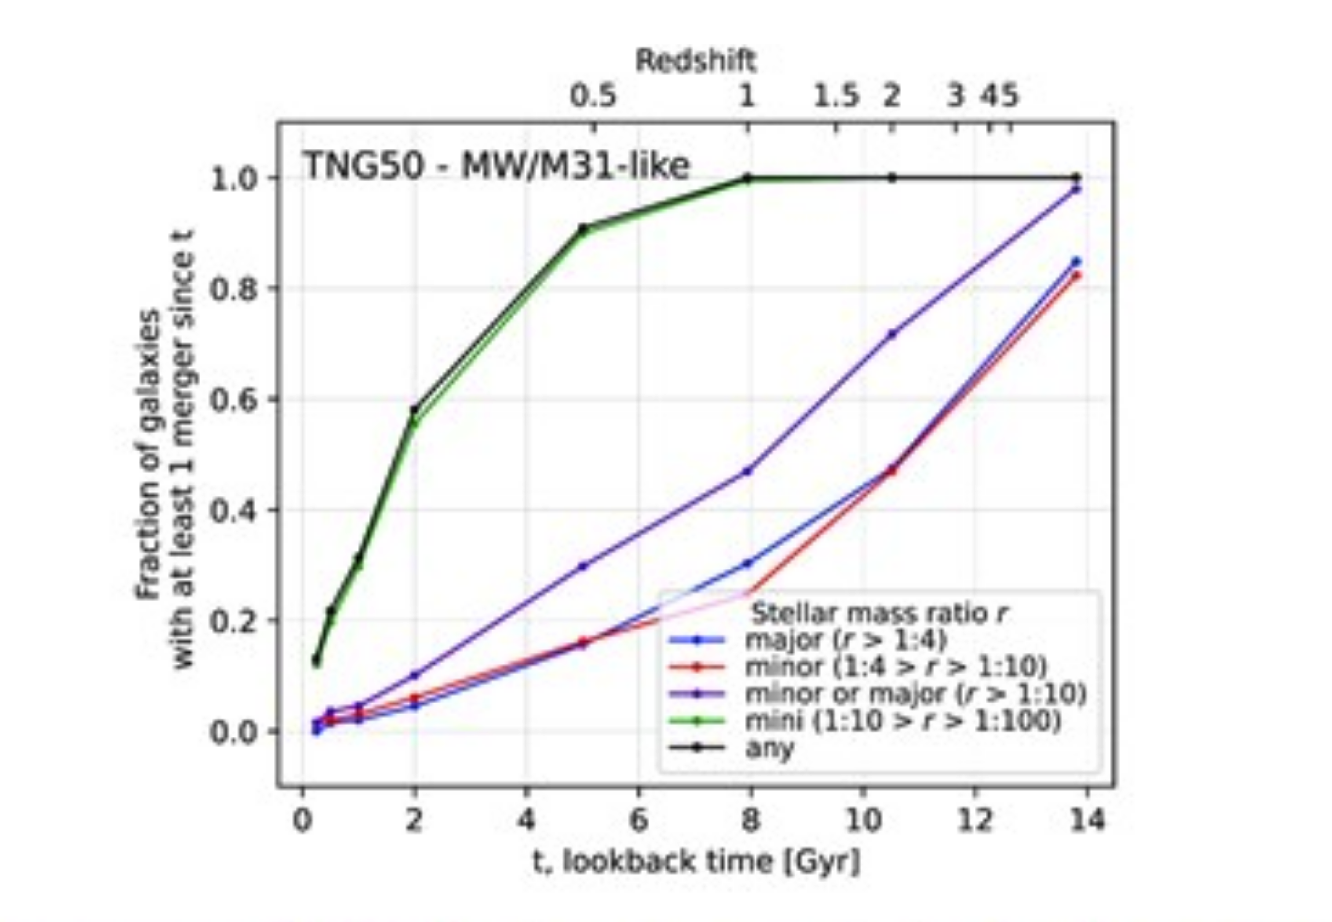
\includegraphics[width=1.2\linewidth]{research assignment 2/Merger_stat.jpeg}
    \caption{Fraction of galaxies with at least one merger versus the lookback time. A major merger, i.e., a merger with a similar massive galaxy, is shown in blue lines. Minor merger, i.e., a merger with a less massive galaxy, is shown in red line, and any merger is shown in black line \citep{Ramos+2022}.}
    \label{fig:merger statistics}
\end{figure}

A leading open question in the Galaxy-Halo connection in stellar remanent is whether the stellar remanent of the merger follows the established SHMR \citep{Moster+2013}. The observed burst in star formation in a merger event may cause a system to deviate from this relation\citep{Hopkins+2010}. An opposing phenomenon, like feedback mechanisms, may force the system to fall back on or deviate further from the relation. Furthermore, how long would it take for the merged system to follow the relation if there is such deviation? One kinematics question would be if the angular momentum of the remanent is conserved in a merger event, and what would the velocity curve of the remanent halo look like? Another intriguing question would be whether the phase space diagram of the halo of the remanent looks any similar to the phase space diagram of either of the parent galaxies prior to the merger.

\section{The proposal}
\subsection{This proposal}
This study will primarily investigate whether the merger's stellar remanent is consistent with the SHMR from collisionless N-body simulations of MW and M31 \citep{Marel+2012}. If time prevails, the study will also try to explain how the net angular momentum evolves before and after the merger. The majority of this proposal, however, will focus on the primary question.

\subsection{Methods}
This study uses the N-body simulations of MW and M31 \citep{Marel+2012}. Since the focus is not on mapping the detailed galactic structure of the merger remnant, the analysis relies on low-resolution simulation data. The primary goal is to determine the stellar and halo mass of the merged remnant and compare it to the 
SHMR. The first part of the study would be to establish the SHMR from \citet{Moster+2013}, as shown in Figure \ref{Moster}, and follows the equation at z = 0:
$$\frac{m}{M} = 2N \left [ \left ( \frac{M}{M_1} \right)^{-\beta} + \left (\frac{M}{M_1} \right)^{\gamma} \right]$$
where, $m$ = stellar mass, $M$ = halo mass
$$\log M_1(z) = M_{10} + M_{11} \frac{z}{z+1}; N(z) = N_{10} + N_{11} \frac{z}{z+1}$$
$$\beta(z) = \beta_{10} + \beta_{11} \frac{z}{z+1}; \gamma(z) = \gamma_{10} + \gamma_{11} \frac{z}{z+1}$$
This study uses the same values of the constants as given in \citet{Moster+2013}.
\begin{figure}
    \centering
    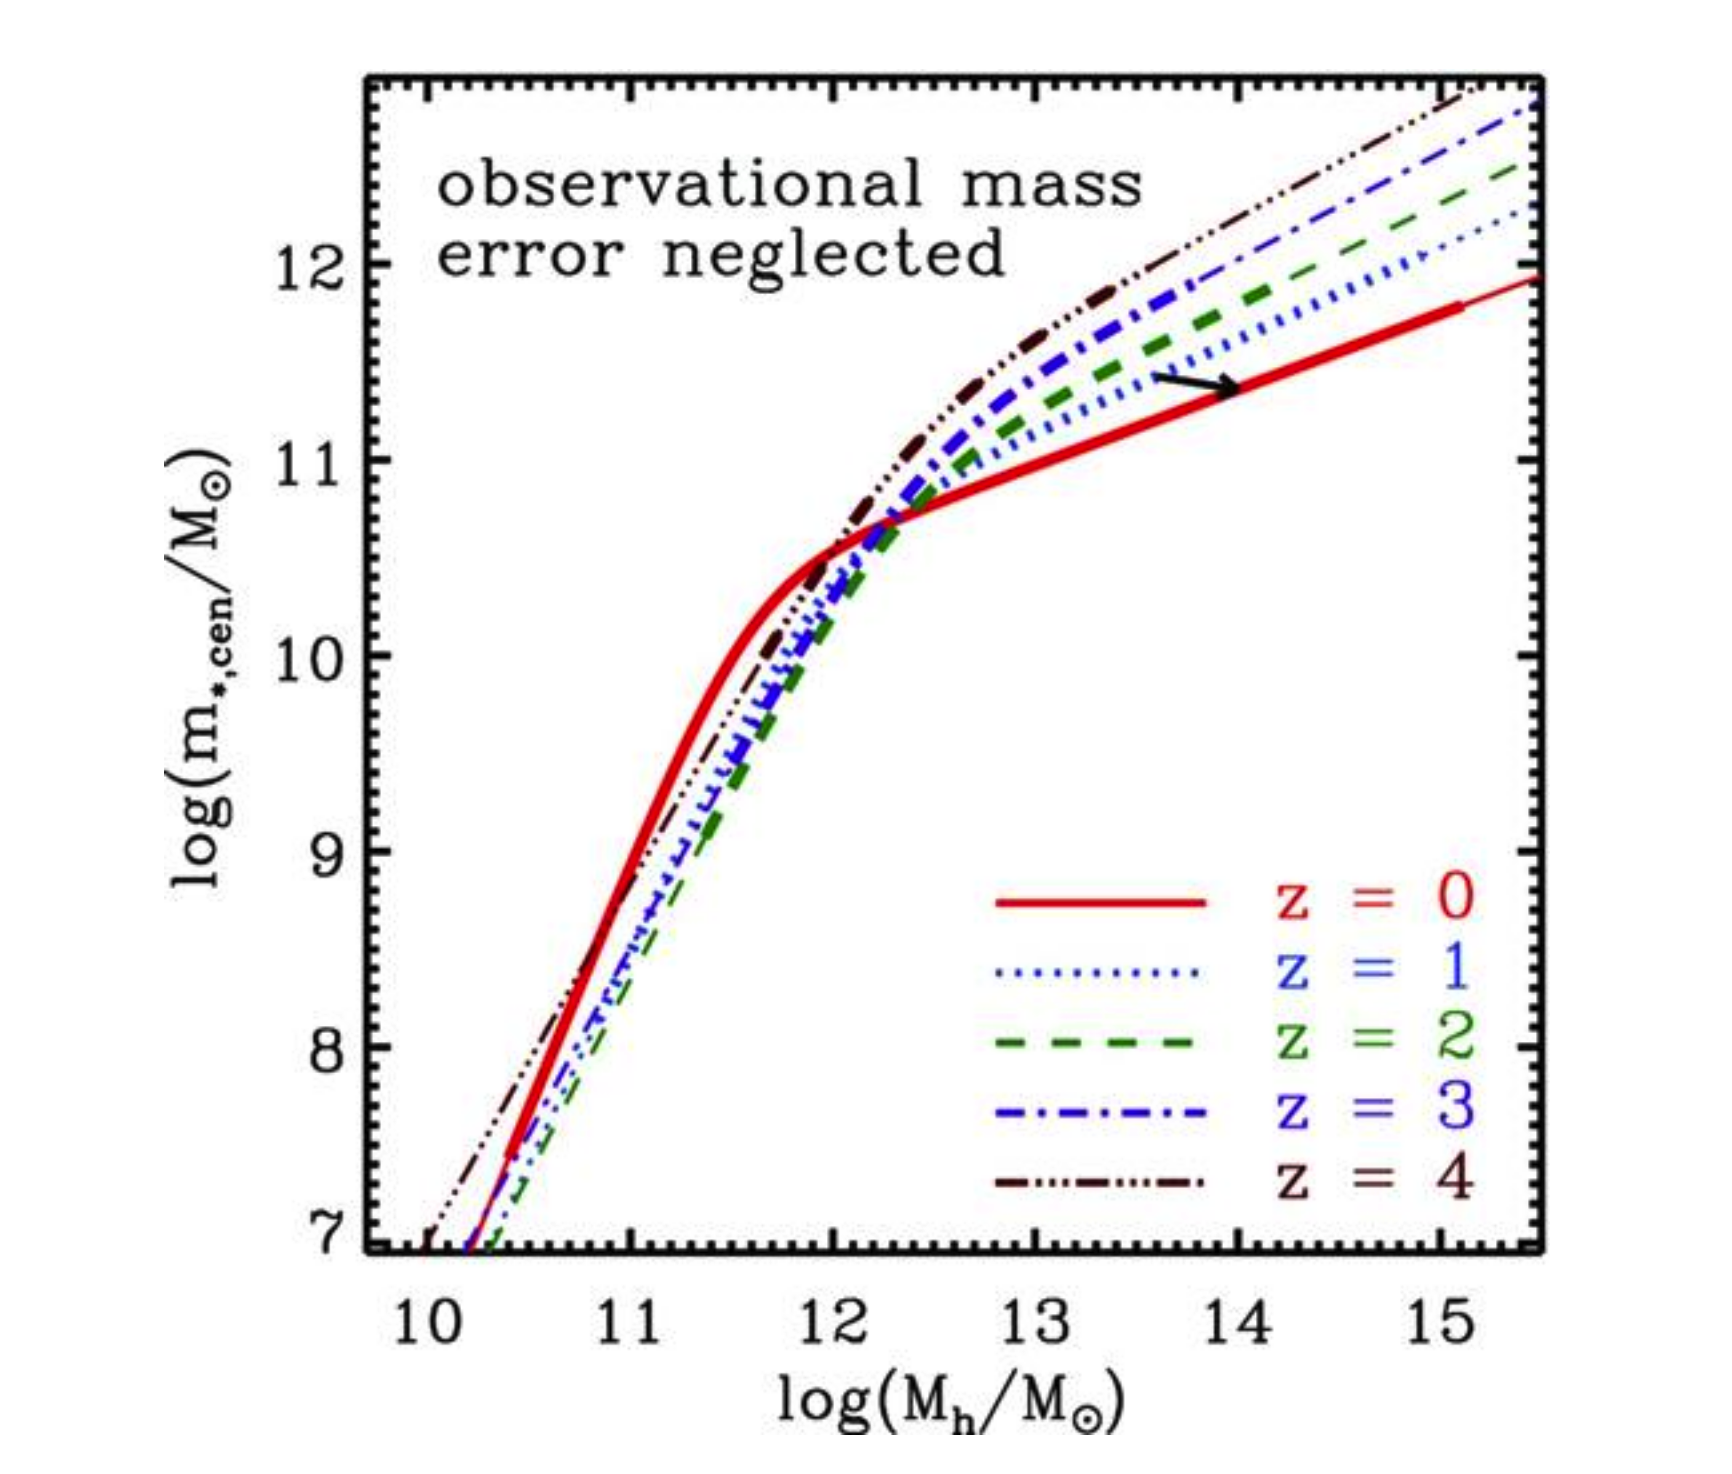
\includegraphics[width=1\linewidth]{research assignment 2/Mosterfin.png}
    \caption{Moster relation, Stellar Halo mass relation as a function of halo mass for different redshifts \citep{Moster+2013}.}
    \label{Moster}
\end{figure}

The next part of the study is to find the halo and stellar mass of the merger remanent of MW and M31. By creating a function that loops over all the snapshots, we can compute the Center of Mass position and velocity as a function of time. This inherently is the orbit of both the galaxies. Here, the Center of mass is computed using the following equation:

\[\textbf{x}_{COM} = \frac{\Sigma x_im_i}{\Sigma m_i}\]
where x is a vector, either position or velocity, and m is the mass of the particle in the simulation.

Next is to find the epoch when the two systems merge. This can be done by creating a function that finds the difference between the magnitude of the relative separation and velocity of the two systems. The first merger occurs when the distance between the two COMs is negligible. This snapshot and all the above will now become our primary data for calculating the remanent's total stellar and halo mass.

This study believes that one specific snapshot may not give much information on where the merger remanent lies on the SHMR, so it would be more beneficial to see how the Stellar mass and Halo mass change with time. So, we will calculate the stellar and halo mass for each snapshot in our primary data. We will calculate the stellar mass using each galaxy's disk and bulge particles and the halo mass by using the halo particles in the simulation.

The last step would be to plot all these values on the SHMR at z = 0 and see how much it deviates. It will be very intriguing to see how the merger remanent looks on the relationship as it evolves over time. Figure \ref{Visualization} illustrates this methodology. 


\subsection{Hypothesis}
I believe that the remanent will deviate from the SHMR, but for the later snapshots, it will start falling towards the relation. I have different reasons for this;
\begin{enumerate}
    \item There might be a starburst due to the collision of gases and the accretion of surrounding gases to the increased gravitational potential well. This will cause the stellar mass to be increased in the earlier epoch of the merger. However, as time progresses, the star formation will slow down and match SHMR relative to the new halo mass.
    \item Earlier stages of tidal stripping may cause the merger remanent to seem deviated. Still, the deviation will decrease as all the tidal debris falls back in and the whole system is in a more equilibrium/stabilized state.
\end{enumerate}
\begin{figure}
    \centering
    \includegraphics[width=1\linewidth]{Note Mar 20, 2025.pdf}
    \caption{Visualization of the methods of this study.}
    \label{Visualization}
\end{figure}


\bibliography{sample7}{}
\bibliographystyle{aasjournal}


\end{document}
